
\section{LSST Operations}
\frame{\frametitle{LSST operations proposal }
\begin{itemize}
\item Proposal was submitted in summer to NSF/DOE to fund LSST operations
\item A joint agency review was completed with positive feedback Dec 7$^{th}$ 2017.
\item LSST Operations key points:
\begin{itemize}
\item Distributed over SLAC, Tucson, La Serena, NCSA Illinois

\item LSST  Sata Facility element
\item To fit in the new National Center for Optical and infrared Astronomy (NCOA) framework
\end{itemize}
\end{itemize}

{\large \color{red} Wht I will present  are elements of the proposal - it is not accepted yet.}


}

\frame{\frametitle{LSST Operations - Distributed}

\begin{columns}
\column{0.2\textwidth}
\vspace {-6cm}
\\
100 - 200\,Gbps international links\\
\vspace{5pt}
40 - 200\,Gbps summit base\\
\vspace{5pt}
See \citedsp{LSE-78}\\
\vspace{15pt}
{\tiny \bf Jeff Kantor }

\column{0.8\textwidth}
\includegraphics[width=1\textwidth]{images/SitesDataflow}\\
\hfill {\tiny \bf Emily Acosta }
\end{columns}
}



\frame{\frametitle{LSST Operations - Organisation}
\includegraphics[width=0.9\textwidth]{images/LSSTopsHighLevelOrg}
{\tiny \bf Beth Willman }
}
\frame{\frametitle{LSST Operations - Communications}

\begin{columns}
\column{0.6\textwidth}
\includegraphics[width=0.9\textwidth]{images/LSSTopsCom}\\
{\tiny \bf Phil Marshall }
\column{0.4\textwidth}
\vspace{-4cm}
\begin{itemize}
\item Formal and informal  channels in place
\item Regular weekly daily meetings as well as Jira for tracking
\item Slack, community.lsst.org, etc as well
\end{itemize}
\end{columns}
}

\frame{\frametitle{Observatory Operations Activities (on summit) }
\begin{columns}
\column{0.44\textwidth}
\includegraphics[width=1\textwidth]{images/summit24hrs}\\
\column{0.56\textwidth}
\vspace{-6cm}
\\
High level 24 hour activity (50FTE):
\begin{itemize}
\item Regular maintenance
\item Evening calibrations
\item Nightly observations
\item Day crew, night crew shift 1, night crew shift 2
\item Software
\item ITC supports daily data transmission
\end{itemize}
\vspace {1cm}
\hfill {\tiny \bf Chuck Claver }
\end{columns}
}


\frame{\frametitle{What is Science Operations ?}
\vspace{-0.2cm}
\center {\bf Deliver the science products defined  \citeds{LSE-163} to the community.}
\begin{columns}
\column{0.5\textwidth}
\vspace{-5.7cm}
\\That entails working with :
\begin{enumerate}
\item Chilean Operations to make sure the observations are scientifically good
\item the Data Facility to ensure production is running correctly
\item Survey performance to make sure over the longer period we will meet science goals.
\item EPO to communicate our successes {\bf and possible more importantly our short comings}.
\end{enumerate}
\column{0.5\textwidth}
  \includegraphics[width=1.0\textwidth]{images/LSSTopsCom}\\
\end{columns}
{\bf \color{red} AND  Maintain/improve software systems bought over from data management}
}


\frame{\frametitle{Science Operations: Curating LSST Science }
On a daily basis Science Operations Staff are looking at data quality from both instrument and software perspectives asking many questions (28FTE):

\begin{itemize}
\item Are the alerts as good as we can make them ?
\item Are there any data products we could deliver/improve?
\item Are the changes we should request on the telescope ?
\item Was there some event (weather/hardware) affecting data we should be telling the community about ?

\end{itemize}
Longer term :
\begin{itemize}
\item Are there any disturbing trends in Key Performance Metrics?
\item How is the Data Release Product quality ?
\end{itemize}
}

\frame{\frametitle{Organization: Science Operations reporting}
\begin{center}
  \includegraphics[width=0.7\textwidth]{images/LSSTopsHighLevelOrg}\\
\end{center}
\vspace{-1cm}
\begin{itemize}
\item Science operations is one of the main pillars of LSST operations
\item FY23 estimate is to have 28FTE in the department
\item going down to  23FTE over 4 years
\end{itemize}
}

\frame{\frametitle{Organization: Science Operations groups}
We are organized into three groups, which parallel the key components of science deliverables:\\

\begin{columns}
\column{0.3\textwidth}
\begin{itemize}
\item  Observatory Science
\item  Science Algorithms and Pipelines
\item Science Platform.
\end{itemize}


\column{0.7\textwidth}
\vspace{-1cm}
\begin{center}
  \includegraphics[width=0.9\textwidth]{images/LSSTSciOpsOrg}\\
\end{center}

\end{columns}
}


\frame{\frametitle{Observatory Science Group}
5.5 FTE starting in Chile to learn the instrument and them migrating to Tucson\\
This group should:
\begin{itemize}
\item   Understand end-to-end impact of hardware and summit conditions on science
\item   Assure  science images can deliver to LSST’s science requirements
\item   Track and document hardware issues
\item   Propose changes to the telescope, instrumentation or software for efficiency

\end{itemize}
}



\frame{\frametitle{ Algorithms and Pipelines Group }
8 FTE in various institutes eventually converging on Tucson.
\begin{itemize}
\item   Tracking and documenting the data product quality for Alert Production using SDQA and other tools;
\item Proposing when changes need to be made to all aspects of the Alert Production algorithms and pipelines (including distribution of alerts and orbits for solar system objects);
\item Proposing when changes need to be made to all aspects of the annual data release algorithms (including calibration, Multifit, and deblender code); and
\item Proposing to accept or reject software changes based on a scientific validation of new algorithms and an understanding of their impact on required computational resources.

\end{itemize}
}

\frame{\frametitle{Science Platform }
4.5 FTE in Tucson
\begin{itemize}
\item  maintain and evolve the Science User Interface

\item maintain and evolve User Services

\end{itemize}
"Science Platform” refers to the functions that will enable the community to conduct analyses and generate new data products, near the data, and will include Jupyter widgets to enable users to use Jupyter notebook with SUI visualization and a set of special visualization templates for interactive Quality Analysis (QA).
}

\frame{\frametitle{Science Operations Staffing }

\begin{columns}
\begin{column}{0.4\textwidth}
28 FTE starting operations going down to 23 FTE over 4 years.\\
\vspace{15pt}
Combination NCOA and SLAC positions.\\
\vspace{15pt}

Initially support also in institutes e.g. Princeton   \\
\vspace{15pt}

\end{column}
\begin{column}{0.6\textwidth}

\vspace{-10pt}
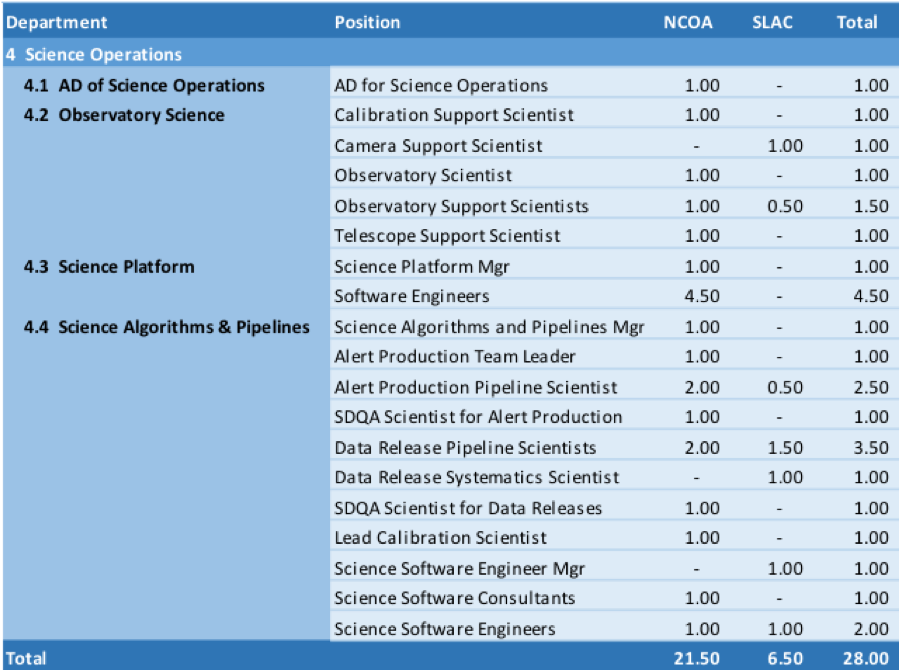
\includegraphics[width=\textwidth]{SciOpsFTE}
\end{column}
\end{columns}

}


\frame{\frametitle{ LSST Data Facility}

\vspace{10pt}
\begin{columns}
\begin{column}{0.4\textwidth}
\vspace{-5.5cm}
\\
NCSA scientific and technical staff drawn from existing core areas of Center expertise. \\
\vspace{15pt}
FNAL due to proximity and existing collaborative relationships (e.g., DES). \\
\vspace{15pt}
SLAC due to intimate knowledge of software created during the LSST construction project. Currently includes QSERV\\


\end{column}
\begin{column}{0.6\textwidth}
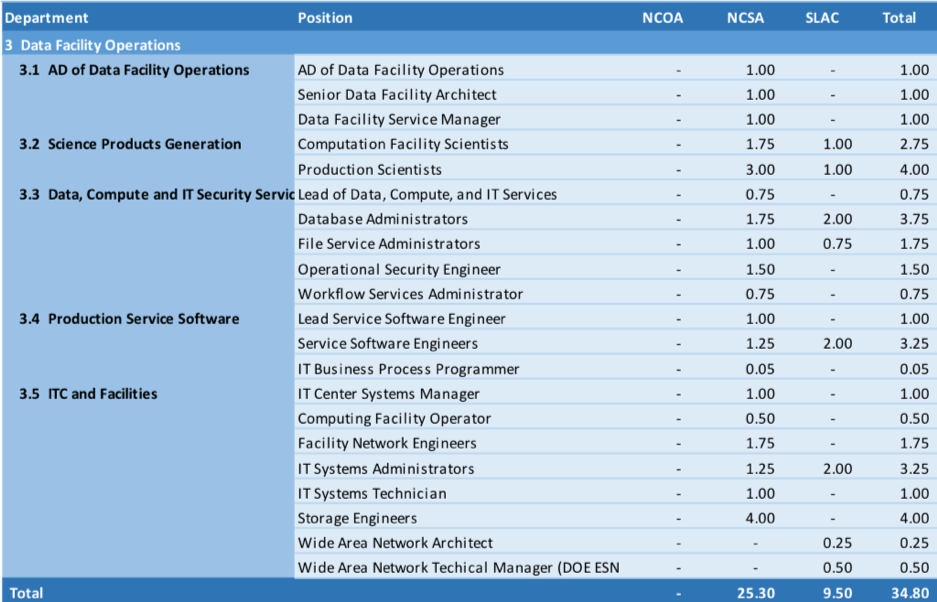
\includegraphics[width=\textwidth]{LDFFTE}\\
\end{column}
\end{columns}

}

\frame{\frametitle{LSST Operations - Proposed Staffing profile}
\includegraphics[width=0.9\textwidth]{images/opsStaffProfile}
}


\section{Commissioning}
\frame {\frametitle{Hopefully {\color{red}not} DM commissioning }
	\vspace{-9pt}
\begin{center}
\includegraphics[width=0.9\textwidth]{images/Raft_of_the_Medusa_-_Theodore_Gericault} \\
	\vspace{-3pt}
{\tiny \bf Raft of the Medusa, Theodore Gericault}
\end{center}
}

\frame{\frametitle{Operations Rehearsals }
\tiny
\begin{longtable} {|l|l|p{0.7\textwidth}|}
	\hline
\textbf{Date/Freq} &\textbf{Location}& \textbf{Title, Description} \\ \hline

Oct 2018 &  NCSA & \textbf{Operations rehearsal for commissioning }
	With TBD weeks commissioning (lets say a week) -- pick which parts of plan we could rehearse.
	Chuck suggests Instrument Signal Removal should be the focus of this (or the next rehearsal).
	\\ \hline
Oct 2019 & NCSA &  \textbf{Operations rehearsal \#2 for commissioning}
More complete rehearsal -- where do the scientist look at quality data? How do they feed it back to the Telescope ?
How do we create/update calibrations ? Exercises some of the control loops.
\\ \hline
Jan 2020 & Base  &  \textbf{Operations rehearsal \#3 for commissioning}
Dress rehearsal -- Just like it will be April for the actual commissioning.
	\\ \hline
Dec 2020 &  NCSA &  \textbf{Operations rehearsal data release processing (commissioning data)}
	Dress rehearsal -- Just like it will be April for the actual commissioning.
	\\ \hline

2021 &  NCSA &  \textbf{Operations rehearsal for data release processing (regular data).}
	\\ \hline

Feb 2022 &  NCSA/Base &  \textbf{Operations rehearsal}
Rehearsals for real operations which start Oct 2022
	\\ \hline
Sept 2022 &  NCSA/Base &  \textbf{Operations rehearsal}
Full Dress rehearsal for real operations which start Oct 2022
	\\ \hline


\end{longtable}

\normalsize
}

\frame{\frametitle{LSST Operations - Construction transition}
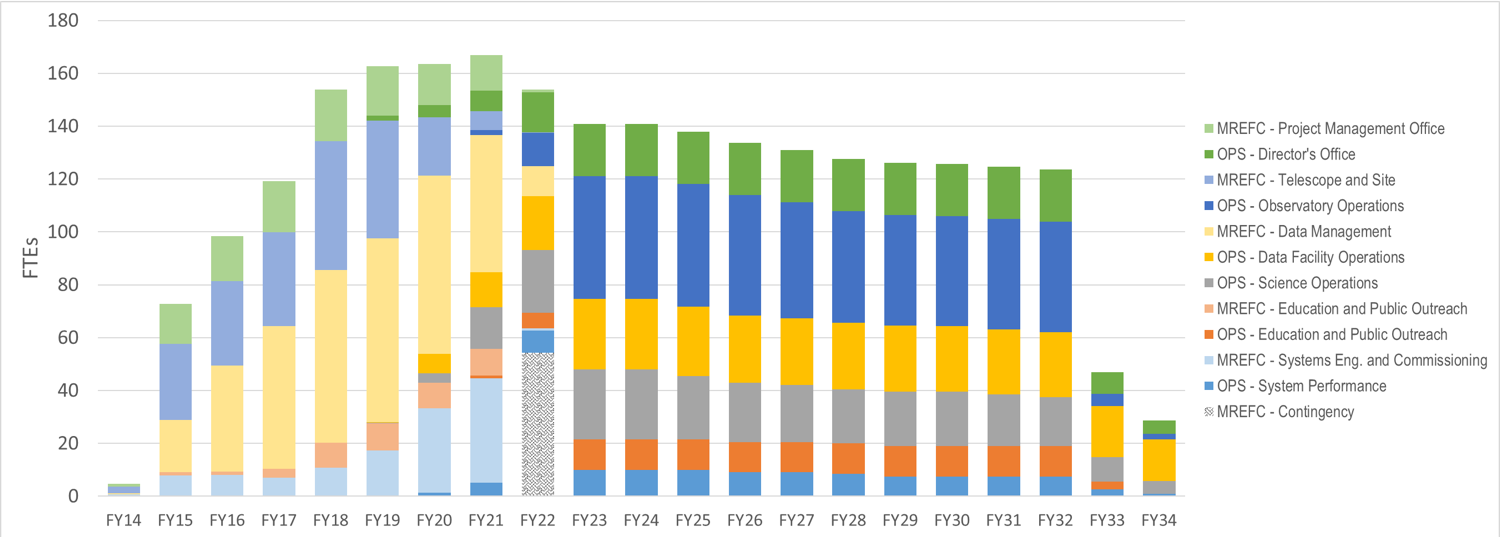
\includegraphics[width=1.0\textwidth]{opsTransFTE}
}


\frame{\frametitle{DM Transition }
\begin{itemize}
\item DM --> Science Operations and LDF
\item Starting to look at specific roles and the transition of DM staff into them
\item  As you see in the previous chart there will be a problem in commissioning to find enough FTEs
\item We may have to extend DM constructing further
\item A few DM people will  be in in Chile for some period of commissioning (Jim, Merlin, Robert \ldots)

\begin{itemize}
\item based on need to see the  hardware
\item  We are exploring this in the commissioning rehearsals
\item Most of us can work from our home institutes or perhaps congregate in Illinois or Tucson for specific events.
\end{itemize}
\end{itemize}
}

